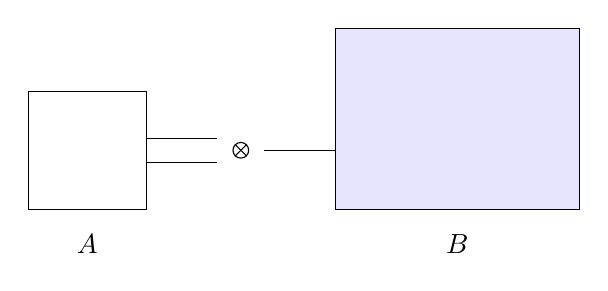
\begin{tikzpicture}[x=1cm,y=1cm,fill=black!12]
  % chamber A (small, left)
  \draw[fill=white] (0,0) rectangle (1.5,1.5);
  \node[below] at (0.75,-0.2) {$A$};
  % connecting tube
  \draw (1.5,0.6) -- (2.4,0.6);
  \draw (1.5,0.9) -- (2.4,0.9);
  % valve symbol: circle with cross
  \node[circle,draw,inner sep=2pt] (v) at (2.7,0.75) {};
  \draw (v.north west) -- (v.south east);
  \draw (v.north east) -- (v.south west);
  \draw (3.0,0.75) -- (3.9,0.75);
  % chamber B (large, right, shaded)
  \draw[fill=blue!10] (3.9,0) rectangle (7.0,2.3);
  \node[below] at (5.45,-0.2) {$B$};
\end{tikzpicture}
